\documentclass{article}
\usepackage{tikz}
\usetikzlibrary{arrows.meta}

\begin{document}

\begin{figure}[h]
    \centering
    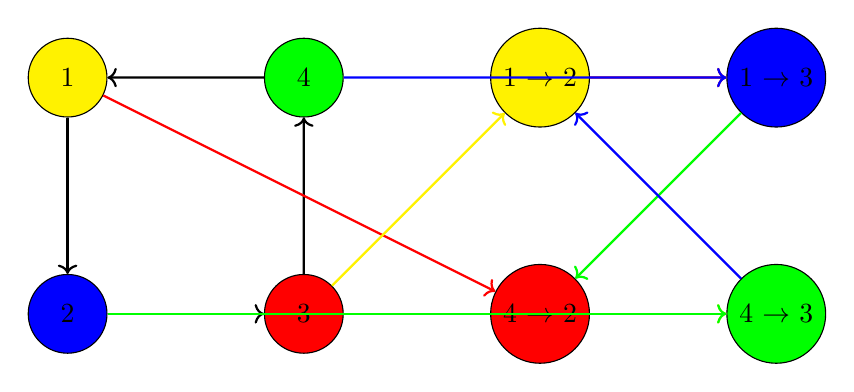
\begin{tikzpicture}[scale=1.5, every node/.style={circle, draw, minimum size=1cm}]
        % Nodes for the left part
        \node[fill=yellow] (1) at (0,2) {1};
        \node[fill=blue] (2) at (0,0) {2};
        \node[fill=red] (3) at (2,0) {3};
        \node[fill=green] (4) at (2,2) {4};

        % Arrows for the left part
        \draw[->, thick] (1) -- (2);
        \draw[->, thick] (2) -- (3);
        \draw[->, thick] (3) -- (4);
        \draw[->, thick] (4) -- (1);

        % Nodes for the right part
        \node[fill=yellow] (1') at (4,2) {1 $\rightarrow$ 2};
        \node[fill=blue] (2') at (6,2) {1 $\rightarrow$ 3};
        \node[fill=red] (3') at (4,0) {4 $\rightarrow$ 2};
        \node[fill=green] (4') at (6,0) {4 $\rightarrow$ 3};

        % Arrows for the right part
        \draw[->, thick, red] (1') -- (2');
        \draw[->, thick, green] (2') -- (3');
        \draw[->, thick, yellow] (3') -- (4');
        \draw[->, thick, blue] (4') -- (1');

        % Edges connecting the two parts
        \draw[->, thick, red] (1) -- (3');
        \draw[->, thick, green] (2) -- (4');
        \draw[->, thick, yellow] (3) -- (1');
        \draw[->, thick, blue] (4) -- (2');
    \end{tikzpicture}
    \caption{An example of the construction in Theorem~\ref{thm:const}. The tournament on the left leads to the coloring of \( V \) on the right.}
    \label{fig:construction_example}
\end{figure}

\end{document}